\section{Сравнение алгоритмов многомерной минимизации}
Алгоритм многомерной минимизации должен отвечать следующим критериям:
\begin{enumerate}
    \item Метод работает для широкого спектра функций. Универсальность метода.
    \item Число необходимых вычислений целевой функции чем меньше тем лучше. Например вычисление одной производной требует 2 вычисления значения функции в разных точках, а второй производной целых 3 значения.
    \item Чем меньше количество итераций для достижения минимума с определенной точностью, тем лучше.
\end{enumerate}

Классическая тестовая задача для проверки алгоритмов многомерной минимизации - функция Розенброка (рис. \ref{fig:Rosenbrock}):
\begin{equation*}
    f(\vec x) = 100 (x_2 - x_1^2)^2 +(1-x_1)^2
\end{equation*}
Известно, что:
\begin{equation}
    \vec x_{min} = \left[\begin{array}{cc}
        1 \\
        1 
    \end{array}\right]\text{;} \qquad f(x_{min}) = 0
\end{equation}
\begin{figure}
    \centering
    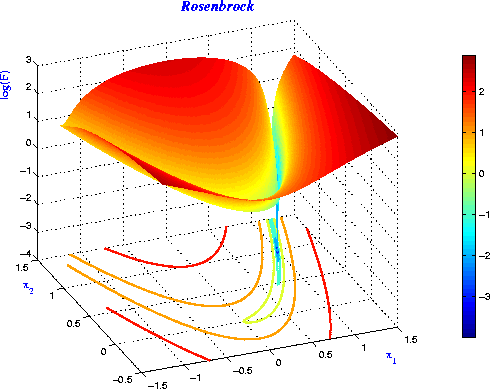
\includegraphics[scale = 0.7]{Pictures/Rosenbrock.png}
    \caption{Функция Розенброка в трехмерном виде}
    \label{fig:Rosenbrock}
\end{figure}
\textit{По аналитическому виду функции можно заметить, что масштаб осей не соразмерен, о чем мы говорили разделе \ref{GradientMethod}}
%Надо изобразить функцию Розенброка

Посмотрим как справятся изученные нами методы с этой функцией (рис. \ref{fig:Rosenbrock_levels}):
\begin{figure}
    \centering
    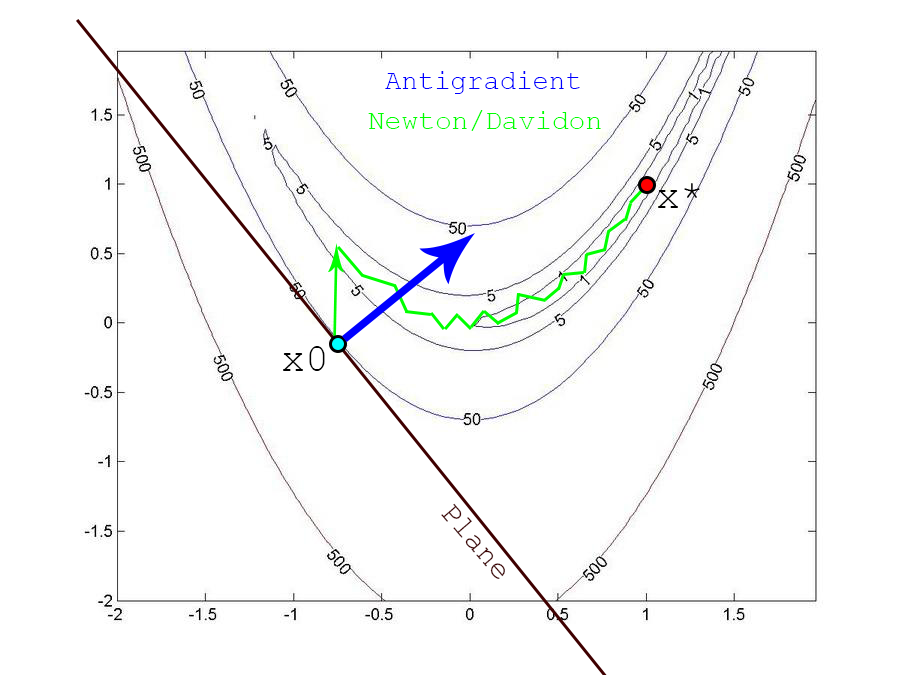
\includegraphics[scale = 0.5]{Pictures/Rosenbrock_levels.png}
    \caption{Линия уровней функции Розенброка. Иллюстрация к сравнению методов.}
    \label{fig:Rosenbrock_levels}
\end{figure}
\begin{enumerate}
    \item Для метода антиградиента может не выйти найти минимум такой функции. Это зависит от первой точки, которая будет выбрана. Минимума мы можем не достичь при выборе точки на левой ветви, поскольку первым шагом мы попадем на <<дно>>, где функция уже мало меняется, и не выполняются критерии продолжения алгоритма. Эта ситуация показывает нам еще один критерий сравнения, а именно независимость от точки старта.
    \item Для метода Ньютона на первом же шаге направление будет отличаться от направления первого шага метода антиградиента, поскольку вторая производная дает методу <<зрение>>. Метод хорошо справляется с тестовой функцией.
    \item Очевидно, что метод Дэвидона тоже справится с такой функцией, поскольку это синтез первых двух методов.
\end{enumerate}
Все программы имеют критерии останова, которые подразумевают, что мы приблизились к минимуму, с достаточной точностью. Однако на деле это не всегда так. Ниже перечислены случаи, когда это утверждение ложно:
\begin{enumerate}
    \item Достижения требуемой окрестности минимума. То есть условия выхода слишком лояльные.
    \item Достигнут локальный минимум. Чтобы избавиться от этого достаточно примерно знать окрестность глобального минимума или повторить процедуру с другой начальной точкой.
    \item Алгоритм толчется на одном месте.
\end{enumerate}

 Однако существуют функции (поверхности) об которые сломается любой из этих алгоритмов. Достаточно посмотреть на рисунки \ref{fig:Bad_surfaces}. Их общая проблема заключается в том, что большая часть функции является просто плоскостью, поэтому здесь алгоритмы минимизации будут бесполезны - программа не сдвинется с места. Однако используя методы Монте-Карло можно <<бросать точку>> по всей поверхности много раз и определить окрестность, в которой функция отлична от константы. В левом рисунке проблема также заключается в том, что в фактическом минимуме функции не существует производной, поэтому рано или поздно двигаясь к минимуму алгоритм сломается.
 \begin{figure}
    \centering
    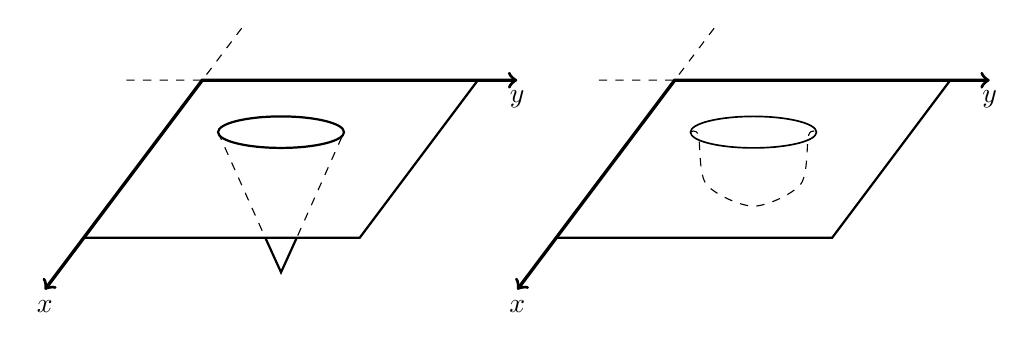
\begin{tikzpicture}
    [scale = 2,
    axis/.style = {<->, very thick},
    dashed line/.style={dashed, thick}]
    \draw[axis](3, 0)node[below]{$y$} -- (1, 0) -- (0, -1.33)node[below]{$x$};
    \draw[dashed](1.25, 0.33) -- (1, 0) -- (0.5, 0);
    \draw[thick](.25, -1) -- (2, -1) -- (2.75, 0);
    \draw[thick] (1.5, -0.33) ellipse (.4 and 0.1);
    \draw[dashed] (1.1, -0.33) -- (1.4, -1) -- (1.6, -1) -- (1.9, -0.33);
    \draw[thick] (1.4, -1) -- (1.5, -1.22) -- (1.6, -1);
    
    \draw[axis](6, 0)node[below]{$y$} -- (4, 0) -- (3, -1.33)node[below]{$x$};
    \draw[dashed](4.25, 0.33) -- (4, 0) -- (3.5, 0);
    \draw[thick](3.25, -1) -- (5, -1) -- (5.75, 0);
    \draw[semithick] (4.5, -0.33) ellipse (.4 and 0.1);
    \draw [dashed] plot [smooth] coordinates {(4.1,-0.33) (4.15, -0.35) (4.2,-0.66) (4.5,-.8) (4.8,-0.66) (4.85, -0.35) (4.9,-0.33)};
    \end{tikzpicture}
    \caption{Поверхности, с которыми методы многомерной минимизации не справятся}
    \label{fig:Bad_surfaces}
\end{figure}
 %Ниже приведу рисунки
 
 \textit{Для экономии вычислительных мощностей и времени работы алгоритмов в физике принято ограничивать значения переменных и функции, в пределах которых ищется минимум.}